\documentclass[12pt, twoside]{article}
\usepackage[letterpaper, margin=1in, headsep=0.5in]{geometry}
\usepackage[english]{babel}
\usepackage[utf8]{inputenc}
\usepackage{amsmath}
\usepackage{amsfonts}
\usepackage{amssymb}
\usepackage{tikz}
\usetikzlibrary{quotes, angles}
\usepackage{graphicx}
%\usepackage{pgfplots}
%\pgfplotsset{width=10cm,compat=1.9}
%\usepgfplotslibrary{statistics}
%\usepackage{pgfplotstable}
%\usepackage{tkz-fct}
%\usepackage{venndiagram}

\usepackage{fancyhdr}
\pagestyle{fancy}
\fancyhf{}

\fancyhead[LE]{\thepage}
\fancyhead[RO]{\thepage \\ Name: \hspace{4cm} \, \\}
\fancyhead[LO]{BECA / Dr. Huson / Geometry 10th Grade\\* Unit 5: Transformation, dilation, \& scale \\ 6 November 2019}

\renewcommand{\headrulewidth}{0pt}

\begin{document}
\subsubsection*{5.2 Do Now: Dilating a triangle, calculating lengths}
  \begin{enumerate}

  \item A dilation centered at $A$ with $k=3$ maps $\triangle ABC \rightarrow \triangle A'B'C'$. Given the sides of the preimage, $AC = 8.5$, $BC = 6.25$, and $AB = 10.5$, find the corresponding lengths of the image, writing your answer showing the multiplication by the value of $k$ using proper notation.
    \vspace{1cm}
    \begin{flushright}
    \begin{tikzpicture}[scale=0.8]
      \draw [-, thick] (0,0) node[above left]{$A'$}--
      (10,0) node[below]{$C'$}--
      (10,7.5) node[above left]{$B'$}--cycle;
      \draw [thick] (4,0)--(4,3);
      \draw [fill] (0,0) circle [radius=0.05] node[below left]{$A$};
      \draw [fill] (4,0) circle [radius=0.05] node[below]{$C$};
      \draw [fill] (4,3) circle [radius=0.05] node[above left]{$B$};
      \node at (2, 0) [below]{$8.5$};
      \node at (2, 2) [above]{$10.5$};
      \node at (4, 1.5) [right]{$6.25$};
    \end{tikzpicture}
  \end{flushright} 

  \item A dilation centered at $A$ maps $\triangle ABC \rightarrow \triangle A'B'C'$. Given the sides of the preimage, $AC = 4$, $BC = 3$, $AB = 5$, and of $B'C' = 7.5$ find the scale factor $k$ and the lengths $A'C'$ and $A'B'$.\\[0.5cm]
  Spicy: Find $CC'$.
    \vspace{1cm}
    \begin{flushright}
    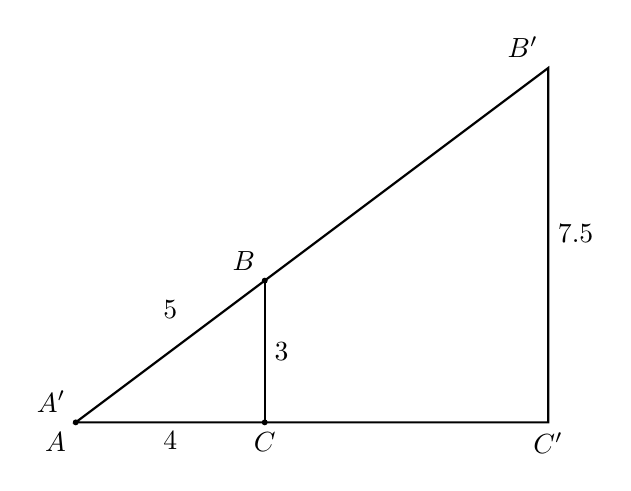
\begin{tikzpicture}[scale=0.6]
      \draw [-, thick] (0,0) node[above left]{$A'$}--
      (10,0) node[below]{$C'$}--
      (10,7.5) node[above left]{$B'$}--cycle;
      \draw [thick] (4,0)--(4,3);
      \draw [fill] (0,0) circle [radius=0.05] node[below left]{$A$};
      \draw [fill] (4,0) circle [radius=0.05] node[below]{$C$};
      \draw [fill] (4,3) circle [radius=0.05] node[above left]{$B$};
      \node at (2, 0) [below]{$4$};
      \node at (2, 2) [above]{$5$};
      \node at (10, 4) [right]{$7.5$};
      \node at (4, 1.5) [right]{$3$};
    \end{tikzpicture}
  \end{flushright} 

\newpage
\item Kevin’s bedroom is 12 feet wide by 8 feet long. His ceilings are 9 feet high.
\begin{enumerate}
  \item If he wants to install carpet tiles that are 1 foot x 1 foot, how many tiles will he need?
  \item Kevin wants to paint the walls (and ceiling), and can cover 100 square feet of wall with 1 gallon can of paint. How many cans of paint will he need? \\
   If each can of paint costs \$10, how much will it cost him to paint his room?
  \item If it takes Kevin 45 minutes to apply each can of paint, how long will it take him to paint his room?
  \item If Kevin invites 2 friends to help him with the job, how long will it take them? \\ 
  (What did you assume to get to this answer?)
  \item Spicy: Kevin’s younger sister Jenny can only paint half as fast as he can. How long will it take the two of them to paint his room together?
  \item Kevin’s air conditioner can reduce the temperature of 2500 cubic feet of air by one degree every 20 minutes. How long will it take to reduce the temperature of his room from 77 degrees to 70 degrees?
\end{enumerate}

\item Kevin’s mom has a room that is 25\% longer and 25\% wider than his room.
\begin{enumerate}
  \item How many carpet tiles would she need?
  \item How many gallons of paint would he need to paint her room?
  \item If she had the same air conditioner, how long would it take to reduce the temperature of her room by 7 degrees?
\end{enumerate}

\item Marcela owns a factory that makes cement blocks. Each block is an exact cube, with each side 2 feet across, and weighs 18 lbs. \\
After the blocks are produced, she needs to store them in a warehouse until they are delivered to her clients.
\begin{enumerate}
  \item She stores them in a warehouse that is 50 feet across and 120 feet long. How many blocks will cover the floor?
  \item If the warehouse is 25 feet high, how many blocks can she hold?
  \item Her old warehouse was 20\% smaller in all dimensions: \\
    What were its dimensions? \\
    How many blocks could she hold there?
\end{enumerate}


\end{enumerate}
\end{document}
